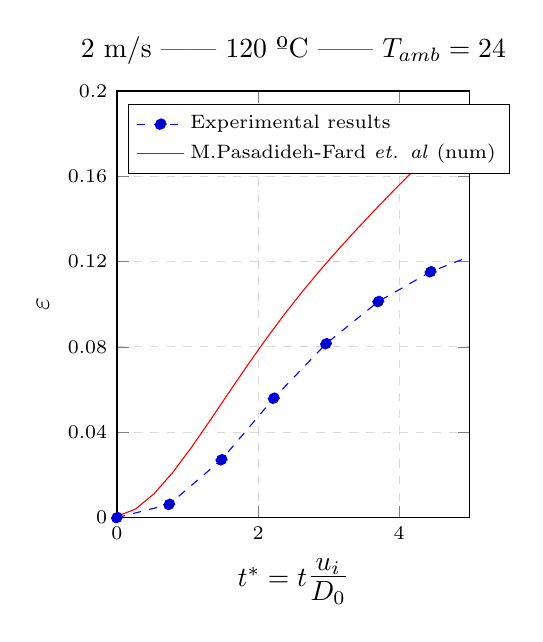
\begin{tikzpicture}
\begin{axis}[
	title = {2 m/s || 120 ºC || $T_{amb}=24$},
    tick label style={font=\scriptsize},
    legend style={font=\scriptsize,/tikz/column 2/.style={column sep=5pt},},
    %legend columns=2,
    legend cell align=left,
	legend pos =north west,
    grid=major, % Display a grid
    grid style={dashed,gray!30}, % Set the style
    xlabel={$t^*=t$\Large{$\frac{u_i}{D_0}$}},
    ylabel={$\varepsilon$}, 
    ymin = 0, ymax = 0.2,
    ytick={0,0.04,0.08,0.12,0.16,0.2},
    yticklabels={0,0.04,0.08,0.12,0.16,0.2},
    xmin = 0, xmax = 5,
    %ytick={0,1600,...,11200},
    %yticklabel style={
    %    /pgf/number format/fixed,
    %    /pgf/number format/precision=5},
	%scaled y ticks=false,
    width=0.5\textwidth, 
    height=7cm,
    cycle list name= color
    ]
\addplot+[dashed]
coordinates {(	0	,	0	)
(	0.740740741	,	0.006183436	)
(	1.481481481	,	0.027132397	)
(	2.222222222	,	0.055947222	)
(	2.962962963	,	0.081489615	)
(	3.703703704	,	0.101288971	)
(	4.444444444	,	0.115230298	)
(	5.185185185	,	0.124822088	)
(	5.925925926	,	0.131242371	)
(	6.666666667	,	0.135432275	)
(	7.407407407	,	0.138496222	)
(	8.148148148	,	0.140580511	)
(	8.888888889	,	0.14177022	)
(	9.62962963	,	0.14257969	)
(	10.37037037	,	0.143075045	)
(	11.11111111	,	0.143348662	)
(	11.85185185	,	0.143623278	)
(	12.59259259	,	0.143854086	)
(	13.33333333	,	0.143895141	)
(	14.07407407	,	0.143929706	)
(	14.81481481	,	0.144092568	)
(	15.55555556	,	0.144183357	)
(	16.2962963	,	0.144236892	)
(	17.03703704	,	0.144266432	)
(	17.77777778	,	0.144186044	)
(	18.51851852	,	0.144202142	)
(	19.25925926	,	0.144378417	)
(	20	,	0.144427272	)
(	20.74074074	,	0.144534209	)
(	21.48148148	,	0.14483881	)
(	22.22222222	,	0.145008105	)
(	22.96296296	,	0.145183721	)
(	23.7037037	,	0.145324486	)
(	24.44444444	,	0.145476178	)
(	25.18518519	,	0.145726953	)
(	25.92592593	,	0.145933468	)
(	26.66666667	,	0.146100459	)
(	27.40740741	,	0.146233525	)
(	28.14814815	,	0.146439453	)
(	28.88888889	,	0.14653441	)
(	29.62962963	,	0.146576075	)
(	30.37037037	,	0.146660443	)
(	31.11111111	,	0.146754592	)
(	31.85185185	,	0.146974795	)
(	32.59259259	,	0.147098626	)
(	33.33333333	,	0.147180226	)
(	34.07407407	,	0.147398825	)
(	34.81481481	,	0.14764873	)
(	35.55555556	,	0.147820618	)
(	36.2962963	,	0.147923815	)
(	37.03703704	,	0.148112059	)
(	37.77777778	,	0.148315615	)
(	38.51851852	,	0.148439	)
(	39.25925926	,	0.148571693	)
(	40	,	0.148709699	)
(	40.74074074	,	0.148776587	)
(	41.48148148	,	0.148849014	)
(	42.22222222	,	0.148966825	)
(	42.96296296	,	0.149264835	)
(	43.7037037	,	0	)
};
\addlegendentry{Experimental results}
\addplot[
    domain=0:5, 
    samples=20,
    color=red,
]{-1.6221*10^(-5)*x^6 + 5.5731*10^(-5)*x^5 + 1.4888*10^(-3)*x^4 - 1.2942*10^(-2)*x^3 + 3.7275*10^(-2)*x^2 + 3.8779*10^(-3)*x + 6.0277*10^(-4)};
\addlegendentry{M.Pasadideh-Fard \textit{et. al} (num)}
\end{axis}
\end{tikzpicture}